\documentclass[runningheads]{llncs}

\usepackage{graphicx}
\usepackage{enumitem}
\usepackage{textcomp}
\usepackage{hyperref}
\usepackage{color,soul}
\usepackage{float}

\usepackage{listings}
\usepackage{color}
\definecolor{gray}{rgb}{0.4,0.4,0.4}
\definecolor{darkblue}{rgb}{0.0,0.0,0.6}
\definecolor{cyan}{rgb}{0.0,0.6,0.6}
\definecolor{yellow}{rgb}{1,1,0.5}
\definecolor{red}{rgb}{1,0,0}
\definecolor{lightred}{rgb}{1,0.5,0.4}



\DeclareRobustCommand{\hlcyan}[1]{{\sethlcolor{cyan}\hl{#1}}}
\DeclareRobustCommand{\hly}[1]{{\sethlcolor{yellow}\hl{#1}}}
\DeclareRobustCommand{\hlred}[1]{{\sethlcolor{lightred}\hl{#1}}}



\setcounter{secnumdepth}{3}
\setcounter{tocdepth}{3}


\lstset{
  basicstyle=\ttfamily,
  columns=fullflexible,
  showstringspaces=false,
  commentstyle=\color{gray}\upshape
}

\lstdefinelanguage{XML}
{
  morestring=[b]",
  morestring=[s]{>}{<},
  morecomment=[s]{<?}{?>},
  stringstyle=\color{black},
  identifierstyle=\color{darkblue},
  keywordstyle=\color{cyan},
  morekeywords={ Description,Tips, BallStartingPosition, SquareStartingPosition, Collectibles, BlackObstacles, GreenObstacles, YellowObstacles, GreenElevators, OrangeElevators, TimeLimit}
}


\newlist{legal}{enumerate}{10}
\setlist[legal]{label*=\arabic*.}


\begin{document}



\title{Procedural Level Generator for Cooperative Games}

\author{Nuno Martins, 83535, nuno.lages.martins@tecnico.ulisboa.pt }

\institute{Instituto Superior Técnico, Lisbon, Portugal \email{mail@tecnico.ulisboa.pt}
\url{tecnico.ulisboa.pt}}

{\def\addcontentsline#1#2#3{}\maketitle}

\begin{abstract}
Procedural content generation has been used in many different ways in video games, but very little has been done in generating content that is specifically aimed at Cooperative games. Therefore we first look at the current state of content generation, such as what types of content can be created and how. We look at how cooperation has appeared in games, from different design patterns to ways of measuring cooperation. Finally we look at an attempt made in creating a generator specifically to cooperative games. Lastly we look at the cooperative game Geometry Friends and propose a way to create a Level Generator for that game.

\keywords{Procedural Content Generation \and Cooperative Game}
\end{abstract}


\tableofcontents
\newpage

\section{Introduction}


\subsection{Motivation}
Procedural Content Generation has been the subject of many studies, this is because it can be a very powerful tool that allows designers the ability to create more in a cost and time effective manner. Cooperation in games has always been considered to be a positive part of gameplay. However the creation of content specifically targeted at cooperation between players has had very little research, so we believe it would be beneficial to improve this area.

\subsection{Goal}

The goal of this work is to create a Procedural Level Generator for Cooperative Games. We hope to be able to apply the knowledge acquired and create a Level Generator for the Cooperative Game Geometry Friends\footnote{Geometry Friends, for more information this is the official website \href{http://gaips.inesc-id.pt/geometryfriends/}{http://gaips.inesc-id.pt/geometryfriends/}}. The generator should be able to receive input from the designer before generating the level. This input should be an abstract representation of a possible solution for a level, such as where should there be cooperative moments or individual moments of gameplay for the players. This input should be given through an editor.

\section{Related Work}

In this section we will define Procedural Content Generation(PCG) and provide a taxonomy for different types of PCG~\cite{ref_togelius}, explore the current state of PCG and define the types of content that can be generated as well as approaches to that content~\cite{ref_hendrikx}. Then we will talk about Cooperation in Video Games, where we explore the description of common Design Patterns in Cooperative Game Mechanics~\cite{ref_rocha}, and define metrics for evaluating cooperation in video games~\cite{ref_magy}.We will also be talking about a study done on the combination of both PCG and Cooperative Games~\cite{ref_arkel} that explorers an approach using level templates.

\subsection{Procedural Content Generation in Games}

Procedural Content Generation(PCG) has been defined as the algorithmic creation of game content with limited or indirect user input~\cite{ref_togelius}, the game Civilization\footnote{Firaxis, 2K Games 2011, Civilization VI, video game, Microsoft Windows, United States.} uses PCG techniques to generate maps, No Mans Sky\footnote{Hello Games 2016, No Man's Sky, video game, Microsoft Windows, United Kingdom.} uses it to create planets and its animals. Togelius et al~\cite{ref_togelius} defined content as most of what is in a game, except things like the game engine and NPC AI (Non-playable Character Artificial Intelligence) behaviour, this definition e too broad so we will define a different one later. 

When developing new tools it is important to be able to classify them, so some desirable properties for a PCG have been defined~\cite{ref_togelius} as:
\begin{itemize}
    \item\textbf{Speed:} can be in real time, meaning while the player is playing, or can be generated beforehand such as during the development of the game and so can take months to generate, or if it is done during a loading screen right before playing in which case it can not be too slow, but does not have to be instant. Therefore the requirements for speed depend on how the content needs to be generated for the game.
    
    \item\textbf{Reliability:} refers to whether the generator is completely random or if it can guarantee certain criteria, for example some generators might not need this quality but others may need to make sure that there is an exit to a dungeon otherwise it is not playable, on the other hand a texture that looks a bit weird is not game breaking.
    
    \item\textbf{Controllability:} If there is something that can be changed, or tweaked by a human to specify certain aspects, this is very important in player adaptive mechanisms. 
    
    \item\textbf{Expressivity and diversity:} the ability to generate levels that aren’t just slight variations on the same thing, but also that aren’t all so different that they become senseless. This is one of the harder properties because of the difficulty of measuring what is expressive or diverse.
    
    \item\textbf{Creativity and believability:} this has to do with whether the generated content can be easily differentiated from human made content or not, mostly we want it to not be obvious.
\end{itemize}

The usefulness of these qualities obviously depend on the game, for example Minecraft\footnote{Mojang 2009, Minecraft, video game, Microsoft Windows, Mojang, Sweden.} requires the generation to be made in real time, as the player moves further away from the starting area the game will generate new environments, as opposed to Terraria\footnote{Re-Logic 2011, Terraria, video game, Microsoft Windows, Re-Logic, Indiana, United States.} where the map is generated once when the world is created, before the player enters the world. When looking at games where cooperation is taken into consideration when creating a level, real time speed can be a requirement that is difficult to meet because there is a need for moments where players have to cooperate in order to progress. For puzzle games Reliability is a necessity, for open world games there can be less of it, for example in Spelunky\footnote{Derek Yu 2008, Spelunky, video game, Microsoft Windos, Derek Yu.} there is a need to guarantee an exit in the each level. Left 4 Dead\footnote{Turtle Rock Studios 2008, Left 4 Dead, video game, Microsoft Windows, Valve, United States.} is a game that experimented with player adaptive mechanisms in a procedural way, they look at the emotional intensity of players and if it is high they remove the generation of threats for some time. Minecraft and Terraria are capable of high level of expressivity with many different maps. Left 4 Dead changes the placement of weapons and the spawn of monsters, this requires a certain amount of believability because it does not make sense to have a monster spawn on top of a building where it can not interact with the player, or weapons appear in non-reachable areas. 

%% There does not seem to be much difference between these dimension and the previous properties
Those properties are not enough to compare different generators so Togelius et al~\cite{ref_togelius} also defined a taxonomy of PCG that consists of the following dimensions:
\begin{itemize}
    \item\textbf{Online vs Offline:} online is the generation of content as the player is playing the game while offline is generating during the development of the game or before the player starts a game session. 
    
    \item\textbf{Necessary vs Optional:} Necessary content is by definition content that is required for completion of a level, while optional is not. This mostly affects the fact that Necessary content needs to be correct, meaning a level must be possible to be completed after generation, while Optional does not. 
    
    \item\textbf{Degree and Dimension of control:} this refers to how the humans can control the generated space, if a seed is used, then using the same seed will generate the exact same level, or a set of parameters can used to have better control on the generation of the content over several dimensions.%%Dimensions here does not really fit 
    
    \item\textbf{Generic vs Adaptive:} Generic methods do not take the players behaviour into account while Adaptive will analyse the behaviour and determine a set of parameters to adapt the generation of content.
    
    \item\textbf{Stochastic vs Deterministic:} Stochastic means that the content generated can not be exactly regenerated, due to the randomness in the generation, as opposed to Deterministic where given the same input it will generate the same output.
    
    \item\textbf{Constructive vs Generate-and-test:} in constructive the generation of the level occurs in one pass while in Generate-and-test it is an iterative process where first a level is generated, then it is tested and then we make adaptations and generate again, until a satisfactory solution is reached.
    
    \item\textbf{Automatic generation versus mixed authorship:} Automatic allows for limited input from the game designer, making possible to tweak some parameters. Mixed authorship tries to allow the designer to give a more abstract input for example drawing part of a 2D level and having the algorithm generate the rest based on constraint satisfaction. 
\end{itemize}

Applying these dimensions to puzzle games, we can see that normally puzzle games have the entire puzzle created beforehand so the content is not generated while the player is playing therefore it is expected an offline approach. Since a puzzle game needs to have a solution the generator has to guarantee that, and since we hope to apply these in cooperative games the generator should also guarantee the necessity for cooperation. When considering the degree and dimension of control it is very dependant on which algorithm is used as basis some allow more or less control and this algorithm will also affect how stochastic or deterministic the generation process is, we explore the different types of algorithms later. If it is possible to define good metrics, that can be tested automatically, then a Generate-and-test approach can help get better levels, possibly ones that have more opportunities for cooperation, however a Constructive approach is just as valid, since in puzzle games the levels can be created beforehand and so the designer can make changes. Since cooperation is a difficult concept to define in an algorithm or through metrics a mixed authorship approach might be able to provide better results. However good results have been achieved with a fully constructive approach~\cite{ref_arkel}.

\subsubsection{Content for Procedural Generation}:
The definition of content by Togelius et al~\cite{ref_togelius} is too broad, Hendrikx et al~\cite{ref_hendrikx} defined content that can be procedurally generated by separating it into layers based on how the content can be created from other content, these layers are: game bits, game space, game systems, game scenarios, game design, and derived content.

\textbf{Game Bits} are the lowest layer and therefore the most elementary units of game content, typically not used to engage the user when considered independently. They can be Concrete or Abstract, Concrete is content that can be interacted with such as trees and items, Abstract is content that needs to be combined to create concrete content such as textures and sound.

Some examples of game bits are:
\begin{itemize}
    \item\textbf{Textures (Abstract):} Images that add detail to geometry and models or visual representation of menus
    
    \item\textbf{Sound (Abstract):} Music is used to set the atmosphere and pace of the game while general sound effects are used as feedback to the player. 
    
    \item\textbf{Vegetation (Concrete):} Adds realism to the game making it more immersive.
    
    \item\textbf{Buildings (Concrete):} Essential for representing urban environments and special buildings often affect the players decision on where to go.
    
    \item\textbf{Behavior (Concrete):} Describes the way in which objects interact with each other and the environment. This helps the game be more interesting.
    \item\textbf{Fire, Water, Stone and Clouds (Concrete):} Help create more believable worlds.
\end{itemize}

\textbf{Game Space} is the environment in which the game takes place, this is partially filled with game bits in which the player is going to navigate. It can also be considered Concrete or Abstract, Concrete spaces tend to closely resemble spaces the way humans perceive them, Abstract is more an imagined space for example the board in the game of chess.

Examples of game spaces are:
\begin{itemize}
    \item\textbf{Indoor Maps (Abstract or Concrete):} Structures and relative position of space partitioned into rooms, that can be connected by corridors, or overlapping and connected by stairs. Can also be caves with varying and unusual geometry.
    
    \item\textbf{Outdoor Maps (Abstract or Concrete):} Can be depictions of elevation and structures of outdoor terrains, normally outdoor maps tend to then have indoor maps.
    
    \item\textbf{Bodies of Water (Concrete):} Can be rivers, lakes and seas and are often used as obstacles or sometimes interactive game space.
    
    \textbf{Other map features (abstract or concrete):} such as teleportation areas and mountains, ridges, ravines, may also be part of game space.
\end{itemize}

\textbf{Game Systems} is a representation of the relation between content in the game, is can be seen as Abstract for example the relation between Vegetation and its relation with to the features of the outdoor maps, or Concrete like cities and networks of cities

Some Examples are:
\begin{itemize}
    \item\textbf{Ecosystems (Abstract or Concrete):} Describes the placing, evolution and interaction of flora and fauna.
    
    \item\textbf{Road Networks (Abstract or Concrete):} form the basic structures of an outdoors map, used for transportation between points of interest
    
    \item\textbf{Urban Environments (Abstract or Concrete):} large clusters of buildings where many people live and interact with their surroundings. 
    
    \item\textbf{Entity Behaviour (Concrete):} Very important for making the player experience in the virtual world life-like. This is done by defining the relation between NPCs and the player including their possible interactions. Hendrikx believes that not only does player interaction requires complex entity behavior but that group movement patterns are examples where procedural algorithms could achieve more realistic results.
\end{itemize}

\textbf{Game Scenarios} describe how the game unfolds. They can describe it in an Abstract way by describing how other objects inter-relate, or in a Concrete way by explicitly showing it to the player as part of the game narrative.

Some Examples are:
\begin{itemize}
    \item\textbf{Puzzles (Abstract):} Are problems that use previous knowledge to be solved or there is a limited amount of possible solutions in which case they can be solved by exploring that finite space i.e. attempting every possible solution.
    
    \item\textbf{Storyboards (Abstract or Concrete):} Are sequential panels describing a scene or event.
    
    \item\textbf{Story (Abstract or Concrete):} Presents the background for the events and goals that the player will go through
    
    \item\textbf{Levels (Abstract or Concrete):} Are normally used as separators between gameplay sequences. They are made by grouping the previous elements and consist of a playable environment that has its objectives, such as solving a sequence of puzzles, or collecting some object.
\end{itemize}

\textbf{Game Design} can refer to all previous types of content including itself, it can be seen as rules or goals, aesthetic components, story or themes.

Part of the game design is:
\begin{itemize}
    \item\textbf{System Design(Abstract):} are the patterns and rules underlying a game.
    
    \item\textbf{World Design (usually Concrete):} is the appearance of the world, when and where the story is taking place and what is the story.~\cite{ref_brathwaite}
\end{itemize}

\textbf{Derived Content} are things that byproduct of the game world. This content helps the player immerse themselves by allowing the player to record their in-game experiences for review inside or outside the game.

For Example:
\begin{itemize}
    \item\textbf{News and Broadcasts (Concrete):} By showing the player or their actions in the news in the game’s universe.
    
    \item\textbf{Leaderboards (Abstract ):} players ranking tables.
\end{itemize}
\subsubsection{Procedural Content Generation Algorithms}:
In this section we will explore different approaches to procedural content generation, and how they can be applied to create the different types of content.

There are many different ways of creating a Procedural Content Generator, Hendrikx et al~\cite{ref_hendrikx} compiled a collection of them and related them to which type of content they could be applied to, first they created a taxonomy to classify the different types of algorithms based on the main basis of the algorithm, this taxonomy identified six groups: Pseudo-Random Number Generators (PRNG), Generative Grammars (GG), Image Filtering (IF), Spatial Algorithms (SA), Modelling and Simulation of Complex Systems (CS), Artificial Intelligence (AI).

%
%\begin{figure}
%    \centering
%    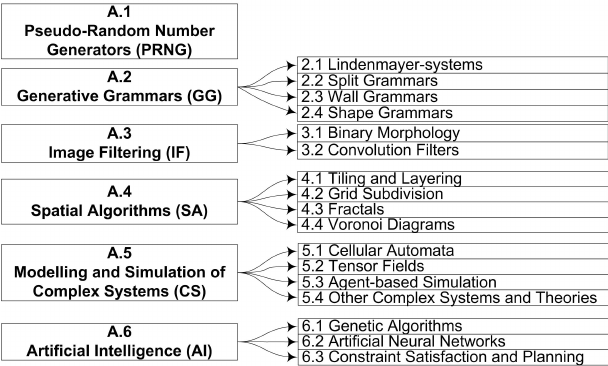
\includegraphics[scale=0.5]{images/hendrikxproceduralmethods.png}
%    \caption{Types of algorithms}
%    \label{fig:algorithm}
%\end{figure}
%

%As seen before each algorithm can be used in many different ways, ahead we will talk a bit about how each work and its usability to our goal.

\textbf{Pseudo Random Number Generators}(PRNG) are algorithms that generate a sequence of numbers that resemble a sequence of random numbers. They are not truly random because the generated sequence is completely determined by an initial value called the seed. Because it has a seed the generation can be reproduced which is very useful for the degree and dimension of control of the generator, and allows for it to be deterministic. 

There are many different ways to generate random numbers~\cite{ref_verth} such as with Linear Congruential methods, Lagged Fibonacci methods, but a very common generator is the Mersenne Twister that has a period of $2^{19937}-1$, this means the it will go back to the initial state and regenerate the same values after $2^{19937}-1$ numbers.

Perlin noise~\cite{ref_perlin} is another of the more common PRNG-based noise generators, it is used mostly for generating textures, fire, smoke, clouds. It generates maps of data points of random values. They are generated by a seeded PRNG through interpolation.

\textbf{Generative Grammars}(GG) consider grammar as a system of rules that through combination of them forms grammatical sentences in a given language. It was originally developed to describe structures in natural languages, phrases, sentences, these are modeled through a set of recursive rules that describes how larger structures are built from smaller ones, for example paragraphs contain sentences, nouns can be a series of other nouns. Individual words are the terminal symbols. They are considered generative because they also describe how to generate them.

Lindenmayer-systems or L-systems is a grammar of symbols that describe the characteristic of an object, they generate strings that describe the structure or behaviour of an object.

Shape Grammars~\cite{ref_stiny} are context-sensitive and sequential grammars that work with shapes as their primitive, ``A shape is a limited arrangement of straight lines in three-dimensional Euclidian space''. By defining a building as a group of shapes, for example a building has an area, then it has floors, windows, doors. Using a grammar syntax we can define how they relate  such as the first floor has a door the other floors have windows and so on, we can then generate a building as can be seen in Figure~\ref{fig:shape}

\begin{figure}
    \centering
    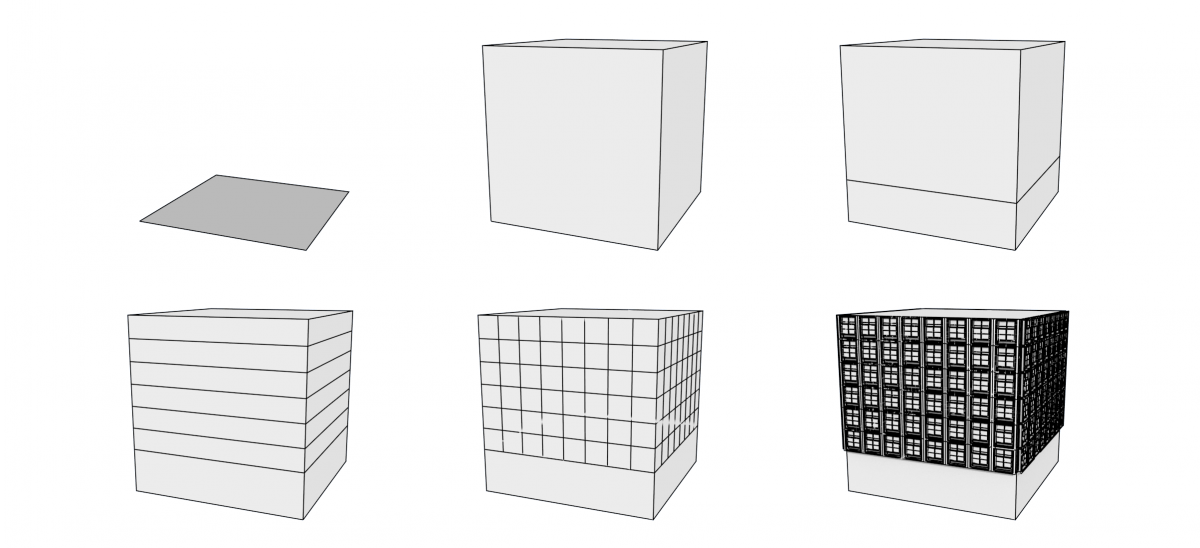
\includegraphics[scale=0.25]{images/shapegrammar.png}
    \caption{Building generated through a Shape Grammar}
    \label{fig:shape}
\end{figure}

Split Grammars~\cite{ref_wonka} also work on string encoded shapes, generating new shapes is done using a basic set of shapes and by applying rewriting rules governing shape-to-shape conversion. These are context-free meaning that the rewriting process always yields the same result given a set of rules, and no matter which order the string is symbols is evaluated.

Wall Grammars~\cite{ref_larive} specifically designed for creating building exteriors, similar to split grammars but can generate more complex shapes.

\textbf{Image Filtering}(IF) algorithms try to improve an image in regards to a (subjective) measure, or to emphasize certain characteristics, such as displaying (partially) hidden information.

Binary Morphology is a set of techniques used for binary operations on images. It uses thresholding, a process where pixels below a certain threshold are set to zero and the rest to one. Common operations are dilation where pixels are added to the edge of an element of an image, another is erosion which is the opposite. More complex operations can be created from simpler ones for example by subtracting from the original an eroded version of it we can get the edges of each element. As can be seen in Figure~\ref{fig:binary} using the kernel s each pixel is put to white only if all surrounding pixels are white, then we can subtract from the original the new image and get the edges of the original.

\begin{figure}
    \centering
    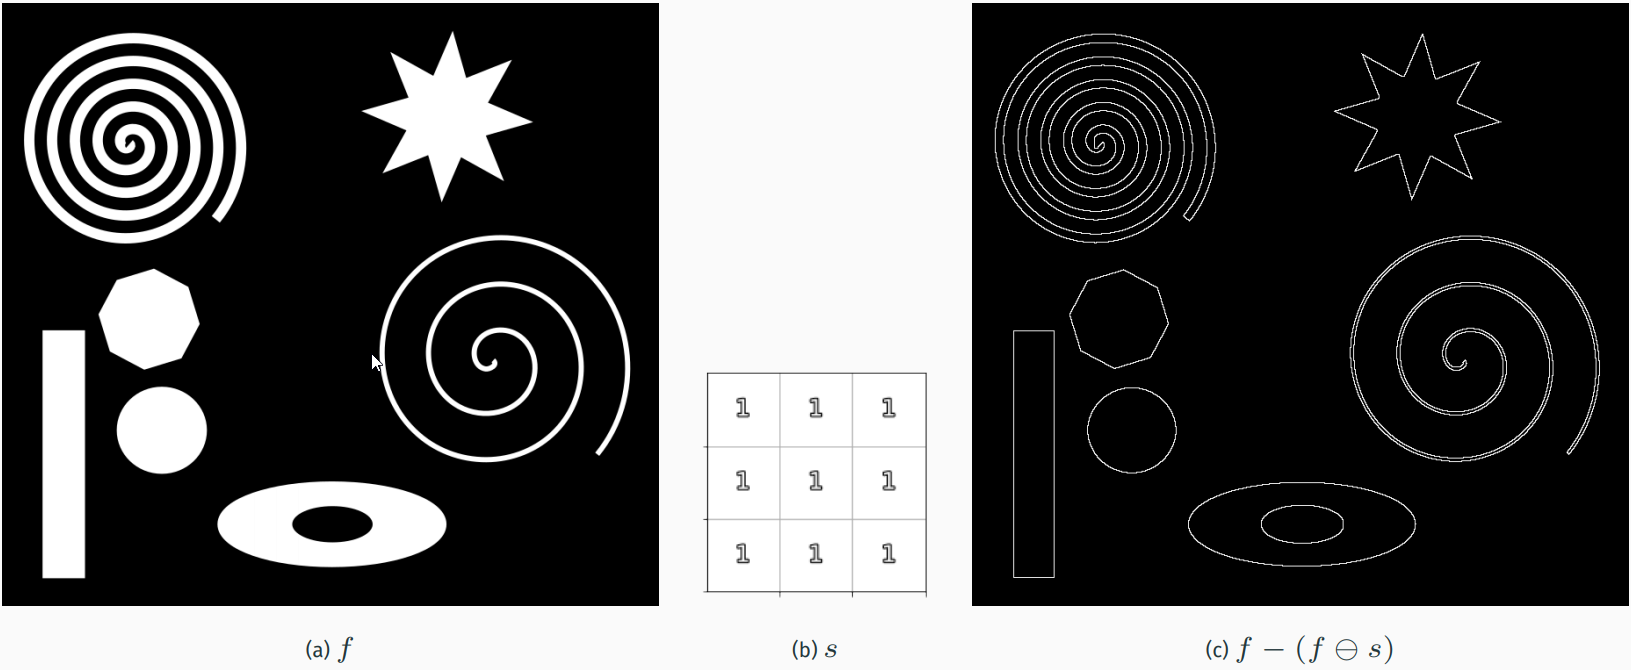
\includegraphics[scale=0.25]{images/binarymorphology.png}
    \caption{Using Binary Morphology for edge detection}
    \label{fig:binary}
\end{figure}

Convolution Filters can be represented by a simple image, for example a matrix representing a kernel(function or discrete data set). Convolution is a mathematical operator on two functions where one function is used to modify the other thereby creating a new function. It can be used to remove noise, smooth, sharpen, detect edges of objects in an image. Using convolution filters, a simple texture can be manipulated to create a whole new texture.

\textbf{Spatial Algorithms}(SA) manipulate space to generate game content, so the input is a structure like a grid.

Tiling and Layering, Tiling is used to create a game space by decomposing a map into a grid. Layering is then integrating into the same map several grids, called layers. A tile then becomes a group of overlapping parts from each layer, some of which may contain transparent parts. This approach enables the creation of overlay effects, such as running water.

Grid Subdivision is an iterative dynamic technique for object generation, it first divides an object into a uniform grid and then for example it is used to add detail to the objects~\cite{ref_pi}.

Fractals are recursive figures which consist of copies of themselves for example a Koch snowflake(a triangle where to each side is added another triangle, and so on for each side of the new triangles). This way objects seemingly have infinite detail that can be stored as a simple recursive function.

Voronoi Diagrams~\cite{ref_franz} are decompositions of metric spaces into parts determined by points of interest, it establishes borders and areas of points equally distant from the closest seed points. The different points (and their areas) can be used to define different countries, vegetation or almost anything. It is not limited to terrain either, it can be used for AI as a kind of influence map, or texture generation.

\textbf{Modeling and Simulation of Complex Systems}(CS) can overcome the difficulties that exist when describing natural phenomena with mathematical equations.

Cellular Automata,~\cite{ref_chopard} a cellular automaton is a discrete computational model based on cells aligned in a grid and each cell has a state that is subject to a set of rules. An initial state is selected by assigning a state for each cell. A new generation is created by advancing the time and according to some fixed rule.

Tensor Fields~\cite{ref_chentensor} are two-dimensional generalizations of vectors used to specify the shape of a game space suitable for interactive design and manipulation of road networks

Agent-based Simulation(ABS)~\cite{ref_davidsson} try to model a complex situation using individuals, the agents, and looks for Emergent behavior, that is, complex behavior that arises from simple interactions.

\textbf{Artificial Intelligence}(AI) is a field  that tries to mimic animal or human intelligence. Examples are speech recognition, planning and execution of tasks by robots.

Genetic Algorithms(GA)~\cite{ref_goldberg} try to solve optimization problems by mimicking biological evolution. They are based on the concept of chromosomes, they represent using a fixed length bit string, where each position is a feature. Then through certain operation, mostly the cross-over operator, where by taking two fit individuals and cross them with one another at a cross-over point, two new “offspring” are generated. Other operations are inversion, where a part of the string is reversed, and bit-flipping mutation where flipping one bit in the string will produce a new offspring. They use a fitness function to determine which offspring should be used to generate new offspring. It ends when the offspring converge, i.e. there is no notable difference between generations, and the use of mutations is to help maintain diversity and keep them from converging prematurely.  

\begin{figure}
    \centering
    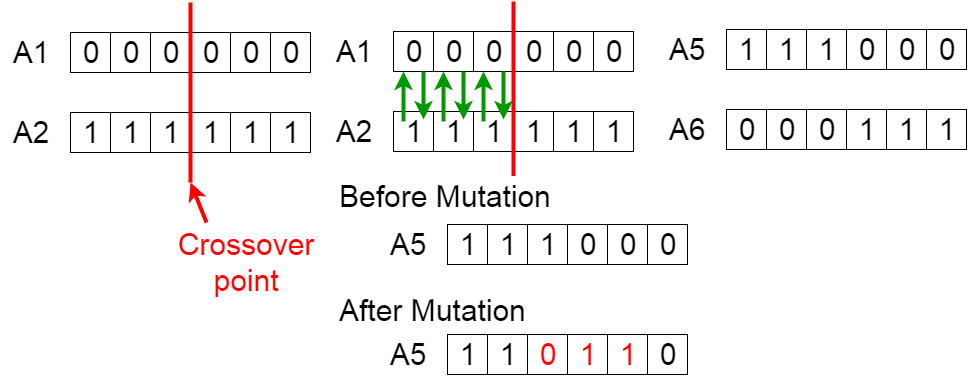
\includegraphics[scale=0.30]{images/geneticalgorithm.png}
    \caption{Generation of new offspring}
    \label{fig:genetic}
\end{figure}

Artificial Neural Networks(ANN)~\cite{ref_haykin} are computational models with the ability to learn the relationship between an input and output. They can be used for finding patterns and classifying, remembering and structuring data.

Constraint Satisfaction and Planning(CSP)~\cite{ref_russel} attempts to find a path from an initial state to an end state by applying actions. A planning problem is an initial state, actions and a goal test.

The most important thing when applying any of these methods in games is that anything that is generated must be playable, meaning must be possible to finish a generated level or a level with generated content.

The different types of content can be generated with different algorithms for example:

Patel~\cite{ref_patel} used an extensive generation process that combines PRNG (Perlin noise), IF (erosion, smoothing), SA (Voronoi diagrams), and CS techniques to generate a complete outdoor map, including an advanced ecosystem.

Some approaches have been attempted to generate System Design for example, The Metagame generator by Pell~\cite{ref_pell}, that generated symmetric chess-like games, another by Togelius and Schmidhuber~\cite{ref_schmidhuber}, uses evolutionary programming to evolve the rules of a PacMan like game and the fitness function is the difficulty to learn. Similarly Hom and Marks~\cite{ref_hom} use genetic algorithms to evolve board games, and the fitness function is based on the balance of the games. Smith and Mateas~\cite{ref_mateas} developed an approach that would automatically test the generated games through a constraint satisfaction technique they named Variations Forever.

Hartsook et al~\cite{ref_hartsook} created a generator that used several of these algorithms to generate a World Design, a Partial order plan as the story, then an adaptation algorithm modifies the story to fit the players preference, then a designer defines a game world model and using this and the preferences, a genetic algorithm creates a 2D Computer Role-Playing Game with the story created by the adaptation algorithm.

Most derived content is generated by the players but Chan et al~\cite{ref_chan} developed a system that generates comics based on key moments in the game session.

\subsection{Cooperation in Video Games}

Cooperation is a concept that has existed for millennia, it is the process of a group working together towards a common goal. Humans enjoy cooperating together so bringing it to video games was expect. Cooperative video games are believed to have started in 1978 with \textit{Fire Truck} arcade game developed by Atari where two players would cooperatively steer the vehicle. Later with the introduction of consoles players would be able to use of multiple controllers, then with the origin of the internet and online multiplayer came the surge of cooperative games like MMORPGs. With the internet there came a need to differentiate between local co-op, where the game is designed for players that are using the same display screen, and online co-op, where each player would use their own screen.

Game theory defines three types of games categories: Competitive, Cooperative and Collaborative. In competitive games players have goals that oppose each other, therefore they need to create strategies that oppose the strategy from the other player, so this types of games are not relevant for our goal.

In Cooperative games both players have different goals but they do not necessarily oppose each other, this means that they may want to help each other in order to get a better result for themselves. These two definitions were part of the traditional Game Theory. Later came the third category Collaborative games. In these games all participants are in a team therefore they all share the outcomes. While participants may have different knowledge and abilities, by sharing the same goal and outcomes they will all have to work together to maximize their utility. So they differ from cooperative games by not forcing the need to cooperate this happens because players have different goals, and therefore different outcomes.

%FOLLOWING PARAGRAPH IS IMPORTANT TO GET RIGHT its about why we do not care about distinguishing cooperative from collaborative
We will not be making this distinguish because in general when we talk about cooperation in video games we do not differentiate between that and collaboration, others, that we will be mentioning ahead~\cite{ref_rocha}\cite{ref_magy}, also do not make that difference so, whenever there is an opportunity for players to work together we consider that as cooperation, whether they have the same or different end goals.

%This might not be a good example
For example in Dead By Daylight\footnote{Behaviour Interactive 2016, Dead By Daylight, video game, Microsoft Windows, Montreal, Canada} the player is part of a team of four that are trying to get away from a monster. The player wins by escaping, to that they need to open the door to escape, before opening it all generators around the map need to be fixed. It is cooperative because some players can distract the monster while others fix the generators, players can save others that have been caught by the monster, and so they need to cooperate, trying to win alone is much harder. However each players end goal is to escape, the others can be caught, as long as they escape, they win.

On the other hand we can look at Overcooked\footnote{Ghost Town Games 2016, Overcooked!, video game, Microsoft Windows, Cambridge, United Kingdom}, or the multiplayer mode from Portal 2\footnote{Valve 2011, Portal 2, video game, Microsoft Windows, Bellevue, Washington, US}. In these games the rewards are shared among the players and so the player wins if the other players also win. However these two are still different types of cooperation, in Overcooked, depending on if the players are completely separated from each other, one player can be enough to finish the level while in Portal it needs both players to complete the level. We consider all these games as cooperative games.

\subsubsection{Game Mechanics for Cooperative Games}:

Cooperation in video games comes in many different ways and Rocha et al~\cite{ref_rocha} defined several common Design Patterns and Challenges Archetypes that appear in video games. These design patterns are:

\begin{itemize}
    \item\textbf{Complementarity:} the most common design pattern, it tries to make sure characters complement each other, by having different abilities of different roles.
    \item\textbf{Synergies between abilities:} Guarantee that the abilities of one  character synergize with the abilities of another character.
    \item\textbf{Abilities that can only be used on another player:} this type of abilities is to incentivize cooperation.
    \item\textbf{Shared Goals:} simple design pattern to make player work together, by giving groups of players goals that are not restricted to one player and therefore can be completed in a group.
    \item\textbf{Synergies between goals (Interlaced/Intertwined goals):} even if players have different goals one approach is to create some sort of synergy between the goals in order for them to cooperate.
    \item\textbf{Special Rules for Players of the same Team:} it is possible that the same action has different outcomes if done on a team member. This can facilitate cooperation.
\end{itemize}

These where later extended by Magy et al~\cite{ref_magy} where they added:
\begin{itemize}
    \item\textbf{Camera Setting:} There are three main ways to have a shared screen in games, split horizontally or vertically, one character in focus, all characters in focus (the screen moves when all characters are near each other). 
    \item\textbf{Interacting with the same object:} providing objects that can be manipulated by abilities from both characters.
    \item\textbf{Shared Puzzles:}to give players a shared challenge of obstacle. 
    \item\textbf{Shared Characters:} providing a character that both players can use but only one at a time, making them discuss how to share the character. 
    \item\textbf{Special characters targeting lone wolf:} having an enemy or obstacle that makes it much harder for a player to work alone, for example an enemy that grapples a player.
    \item\textbf{Vocalization:} having player characters inside the game give feedback of nearby dangers or points of interest.
    \item\textbf{Limited Resources:} limiting resources so that players have to share and exchange their own resources.
\end{itemize}

Reuter et al~\cite{ref_reuter} and Hullettand and Whitehead~\cite{ref_whitehead} also use patterns for describing cooperation, but instead of the patterns describing game mechanics they describe gameplay sections, for example a pattern that describes a segment of the level as: the players have to both interact with two different buttons at the same time, this pattern could then be called Timed Two Man Rule\footnote{The two-man rule is a control mechanism that to give access to actions it requires the presence of two people.}. This is useful because by defining them this way we can look at a level as a sequence of these patterns. 

\subsubsection{Improving Cooperation in Games}:
Zagal et al~\cite{ref_zagal} explored cooperation in board games, however they decided to use the term collaboration instead because they believed that using game theory's definition then cooperative games would still look for only one winner, in which case cooperative games could promote anti-collaborative practices, such as free riding, when a player does not work as much but still benefits, and backstabbing, which is when another player cooperates with another but then that other player defects allowing them to gain an advantage.

For this study they looked specifically at the Lord Of The Rings game by Reiner Knizia. This board game is about getting the hobbit that is carrying the ring from one side of the board to the other before they are corrupted and caught by Sauron, when a player is caught they are removed from the game. The players draw tiles and play cards to advance on the board, they then can choose to draw cards or reduce their state of corruption, if a player plays their last card they increase their state of corruption. Analysing this game they concluded four lessons and three pitfalls that they extended to other cooperative games.

\textbf{Lesson 1:} ``To highlight problems of competitiveness, a collaborative game should introduce a tension between perceived individual utility and team utility."

This lessons tries to address selfish behaviour that affects the team. For example a player draws a tile where he can choose between increasing his corruption by 2 or increasing every players corruption by 1. We can look at individual utility as either increasing corruption by 2 or 1, but when looking at team utility in a team of 5 players it becomes increasing corruption by 2 or 5. A selfish player will choose to have his individual utility be 1 while the teams utility be 5.

\textbf{Lesson 2:} ``To further highlight problems of competitiveness, individual players should be allowed to make decisions and take actions without the consent of the team."

\textbf{Lesson 3:} ``Players must be able to trace payoffs back to their decisions."

\textbf{Lesson 4:} ``To encourage team members to make selfless decisions, a collaborative game should bestow different abilities or responsibilities upon the players."

Although these lessons can be used when designing a cooperative level generator they are more centered in game mechanics and are more useful for designing a cooperative game in itself.

\textbf{Pitfall 1:} ``To avoid the game degenerating into one player making the decisions for the team,collaborative games have to provide a sufficient rationale for collaboration."

\textbf{Pitfall 2:} ``For a game to be engaging, players need to care about the outcome and that outcome should have a satisfying result."

This pitfall obviously applies to all games, but more so to cooperative games, if players are not motivated they will not care enough to help each other, and if the outcome is boring or unrelated to the actions, i.e. a random outcome, then they wont want to learn the consequences of their actions.

\textbf{Pitfall 3:} ``For a collaborative game to be enjoyable multiple times, the experience needs to be different each time and the presented challenge needs to evolve."

The first pitfall is in a way related to how information is portrayed in a game, this is important to take into consideration because a level is a visual representation of information, so a generator has to take into consideration how to show the level, beyond making it playable. The third pitfall is the one we are directly addressing by creating a procedural content generator.

\subsubsection{Evaluating Cooperative Games}:
Magy et al~\cite{ref_magy} defined Cooperative Performance Metrics(CPM), these are associated with observable events, they used them to analyse play sessions for different cooperative games, such as Rock Band 2, Lego Star Wars, Kameo, and Little Big Planet. The final set of CPMs they developed where:
\begin{itemize}
    \item\textbf{Laughter or excitement together}, which is associated to events where players laughed due to a game event, or verbally expressed their enjoyment, or their facial expressions showed happiness or excitement.
    
    \item\textbf{Worked out strategies}, this is associated to talking about how to solve a challenge or how to approach a challenge.
    
    \item\textbf{Helping}, is for when a player indicate to the others how to do something, such as how to use a controller, what is the correct path to solve the puzzle, or saved the other while they were failing.
    
    \item\textbf{Global Strategies}, this metric is related events where players had different roles, for example while one traverses the level the other fights enemies.
    
    \item\textbf{Waited for each other}, was associated to when a player had to wait for another, this was normally due to different levels of skill between the players.
    
    \item\textbf{Got in each others’ way}, is a associated to moments where players wanted to, or did different actions that opposed or hindered progress, or for when one players leads the way and the other lags behind.
\end{itemize}

For their study they had a group of players play cooperative games and recorded their front and back. Then Magy et al analysed the footage, counting all occurrences of these metrics.

These allowed them to better compare games in terms of how cooperative they were, the more positive CPMs the more cooperative a game would be. These metrics can be applied to compare generated levels to non generated ones when user testing, thus giving us a new way to evaluate how cooperative a generated level is.

\subsection{Procedural Content Generator for Cooperative Games}

There are Generators that create maps and levels that allow for multiple players, however these levels are generated based on a single player perspective. Games like Minecraft, Risk of Rain\footnote{Hopoo Games 2013, Risk of Rain, video game, Microsoft Windows, Chucklefish}, use procedural generation to create their maps and levels, they then allow multiple players on these maps, however they are created in a way that does not focus on providing challenges that require cooperation.

Minecraft can be made easier with multiple players, each working on their part of a building, gathering resources or exploring new areas. Risk of Rain follows the same patterns and provides challenges that Rocha et al~\cite{ref_rocha} would classify as Shared Goals. However these are goals that are meant to be achievable alone.

The area that combines both Procedural Content Generation and Cooperation has not had much research, van Arkel et al~\cite{ref_arkel} used PCG to generate levels for a simple cooperative game. Their game is a 2D puzzle-platform game for two players, the objective is to move from the start to the end of a level. The players can move, jump, stand on top of each other and interact with levers or move objects.

They use the term collaborative instead of cooperative because they followed the same definition as Zagal et al~\cite{ref_zagal}, but as mentioned previously we consider both to be interchangeable. 

Van Arkal et al~\cite{ref_arkel} defined game design patterns and for that they followed Reuter et al~\cite{ref_reuter} and Hullettand and Whitehead~\cite{ref_whitehead} approach of having design patterns describe sections of gameplay, this way all a generator had to do would be to combine them and generate gameplay situations.

The patterns they defined are:
\begin{itemize}
    \item\textbf{The Upsy-Daisy:} An obstacle is unreachable by a normal jump and so the players need to time their jumps, with one on top of the other, to reach the object and push it down.
    \item\textbf{Timed Lever-and-Gate:} A lever that when activated opens a gate for a limited amount of time.
    \item\textbf{Common Enemy:} An enemy that has the side facing the player invulnerable to attacks and so one player must distract it so the other can attack it from behind.
\end{itemize}

Van Arkel et al~\cite{ref_arkel} used Ludoscope~\cite{ref_dormans} an AI assisted mission and level design tool, it uses graphs of tasks to determine which tasks are reachable after completing other tasks and which goals become unreachable, it can also determine deadlocks. With Ludoscope it is possible to define the process of generating a level, by breaking it down into steps that can be executed separately, and then it uses the principles of model driven engineering and generative grammars to generate levels.

Their level generation process focus on a more automatic approach, as opposed to a mixed authorship, and so does not include much human interaction. It is based on a sequence of steps: Path Generation, Define Level Segments, Apply Design Patterns, Final Adjustments.

It uses a sequence of generative grammars the first receives a small 6x3 grid of undefined tiles where in the leftmost column they place at random a `Start' tile and then they place at random an `End' tile on the rightmost column.

The Path generation uses two grammars, the first creates a path from left to right, from the start to the end tile, they then move the `End' tile and using the second grammar create a path from right to left. This path is generated by replacing the undefined tiles with tiles that have certain orientations for example `1H' represents horizontal segment `1V' a vertical one, `LCD' stands for Left Corner Down meaning that in that segment the player enters from the left side and would have to move through a corner that exits on the right. They have others like UCR stands for Up-CornerRight, DCR for Down-Corner-Right, \ldots~.

The Define Level Segment expands the smaller grid into a new one where each tile is now 20x20 tile `segment', it is then chosen a template for each segment depending on their orientation, each orientation has several templates. Each template can then have `Encounters' added to them, these are the Game Design patterns described before, `The Upsy-Daisy', `Timed Lever-and-Gate', `Common Enemy'.

The Apply Design Patterns then uses these encounters as smaller level segments to contain the challenges involving certain mechanics. An encounter can have another encounter in it. 

The Final Adjustments corrects some objects orientation, and removes unnecessary information. This level is then put through a parser that reads the Ludoscope output file and using the tiles, their position and type the corresponding objects are placed in Unity.

This approach managed to generate many different levels for their puzzle platform game, however it does not allow for much input beforehand from the Game Designer.

Given that the levels generated use templates for each sections and for the challenges, they can generate many different levels however they can become repetitive if they have a small number of templates. These templates are where the game designers have more control when it comes to the level generation.

\section{Geometry Friends}



Here we talk about the game Geometry Friends\footnote{Geometry Friends,  \href{http://gaips.inesc-id.pt/geometryfriends/}{http://gaips.inesc-id.pt/geometryfriends/}}, where we will be testing our approach, and the two studies done to create a Cooperative Procedural Level Generator also using Geometry Friends as the testbed. First we describe what the game is and what is a level, then we look at how a generator might be created for the game, and look at the attempts made
. 
\begin{figure}
    \centering
    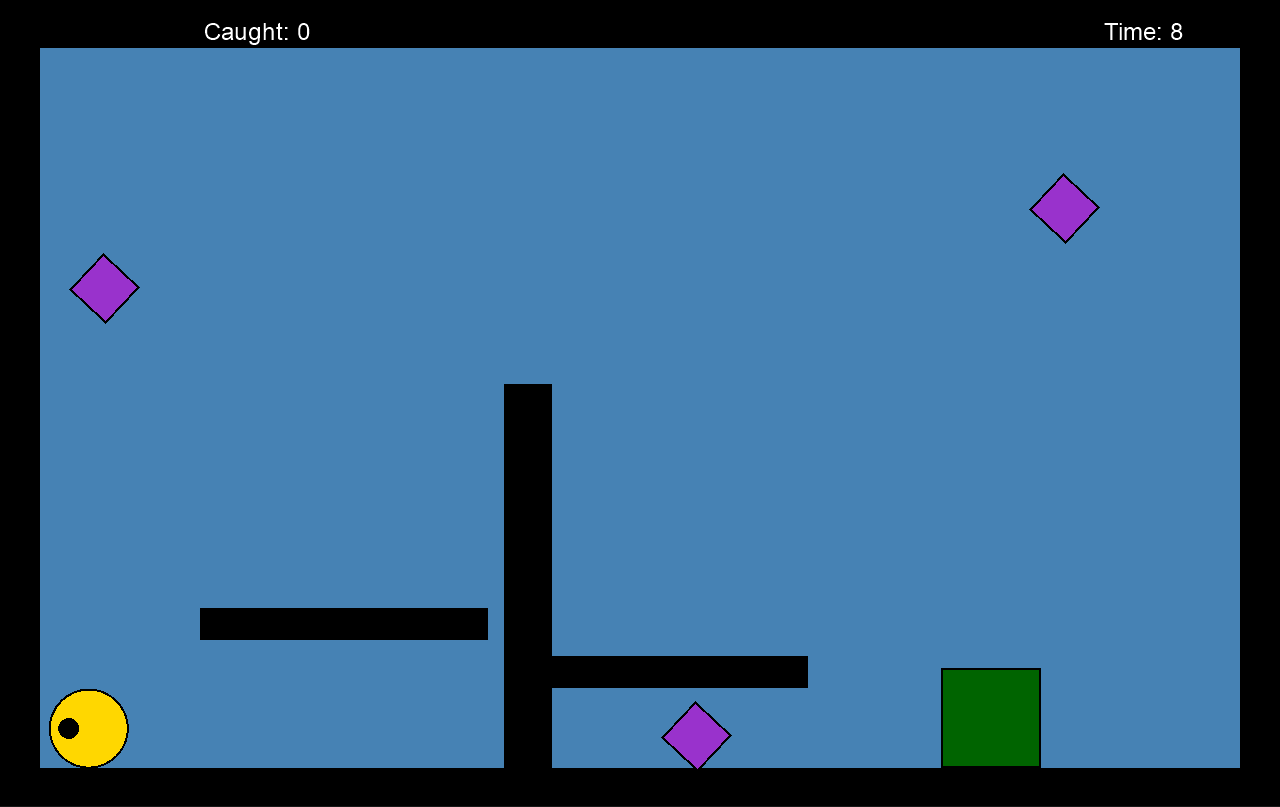
\includegraphics[scale=0.25]{images/levelexample.png}
    \caption{Level in Geometry Friends}
    \label{fig:level}
\end{figure}

Geometry Friends is a cooperative puzzle platform game for two players. The game has two different characters, a yellow circle and a green rectangle. Both characters are subjected to gravity and friction, however, the circle can jump and the rectangle can change its shape to an horizontal or vertical rectangle (with the same area), this difference is where the core gameplay lies. The game is a series of levels with differing difficulties where each level has multiple platforms and the goal is to collect all the purple diamonds, some platforms are colored yellow or green and as such the characters that are not those colors cannot pass through them, some of those colored platforms also move making them elevators. Figure \ref{fig:level} is an example of a level.



\subsection{What is a Level in Geometry Friends?}

What is a level to a player, it is a limited space with walls surrounding it, any number of platforms, and at least one purple diamond to collect, where any diamond that exists must be reachable. There are also the starting positions, one for the circle and another for the rectangle.

If we where to look at a level in a more abstract sense then we can see it as a set of sequences of moves that each character can make in order to complete the level, for example the circle can get on top of a specific platform by jumping and then jump again to pick up a diamond, the rectangle can extend horizontally to pass through a small space then move inside to grab a diamond. This way we can describe a cooperative action as a sequence of timed actions, for example, first the rectangle moves underneath a certain diamond, then extends horizontally, to make it easier for the circle to get on top, second the circle gets on top of the rectangle by moving and jumping, third the rectangle extends vertically to its full height, fourth the circle jumps to reach the diamond. For example figure \ref{fig:levelsolution}. 

\begin{figure}
    \centering
    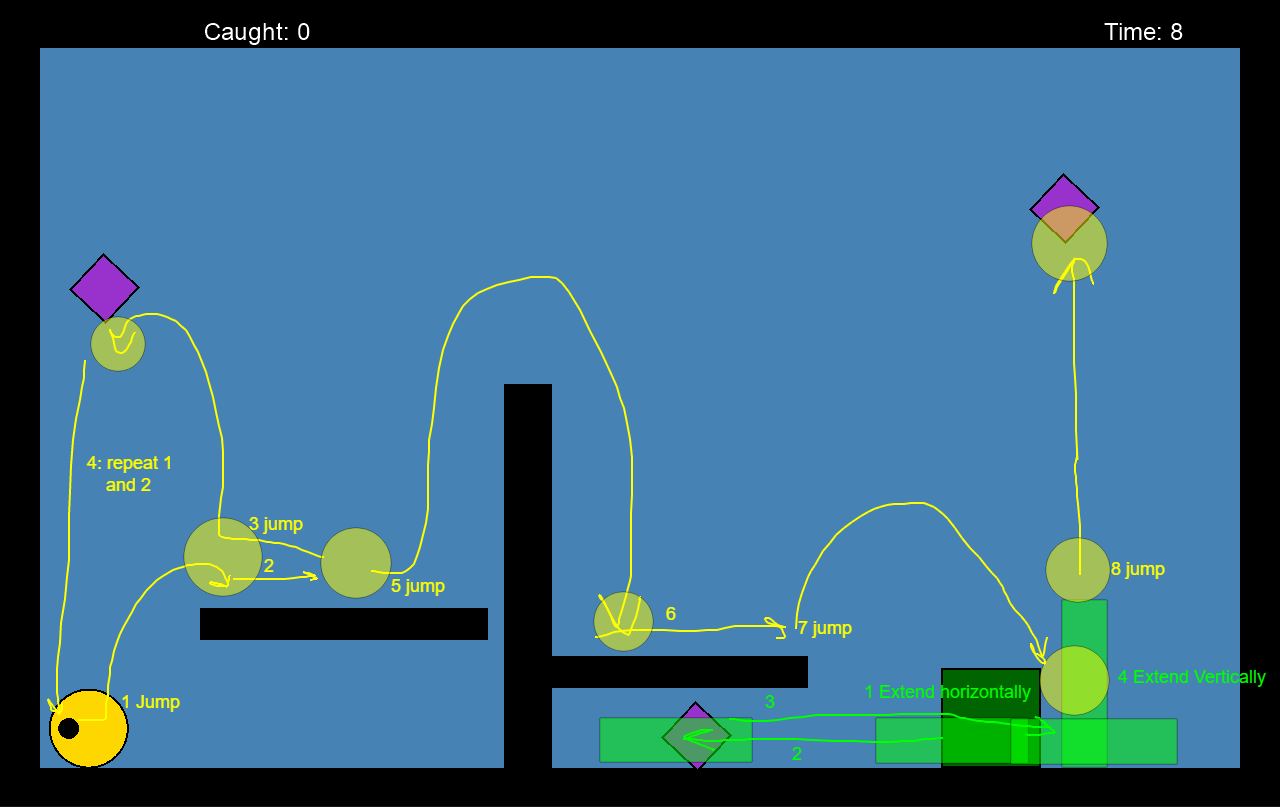
\includegraphics[scale=0.20]{images/levelexamplesolution.png}
    \caption{Possible Sequence of moves to complete the level}
    \label{fig:levelsolution}
\end{figure}

These actions can be seen as all happening in a contained area related to the diamond we are trying to reach, so we could say that, for each diamond we have an area that is classified on who can reach it, this would lead to four different areas: the circle only area, the rectangle only area, the cooperative area, and the common area. In the first only the circle is capable of reaching the diamond, the second only the rectangle is capable of it, in the third both are required in order to reach it, and in the last one both can reach it. For example figure \ref{fig:levelareas}

\begin{figure}
    \centering
    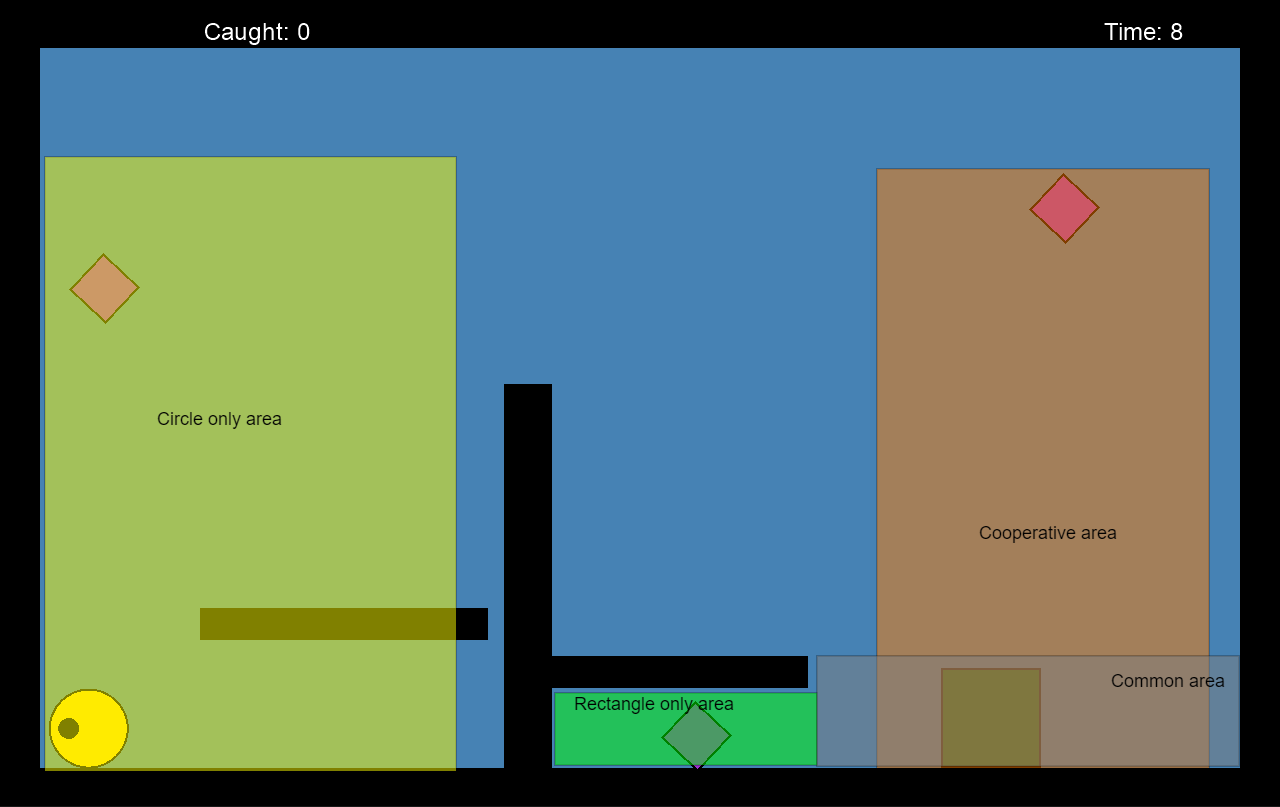
\includegraphics[scale=0.20]{images/lelvelexampleareas.png}
    \caption{Level divided into areas}
    \label{fig:levelareas}
\end{figure}

Geometry Friends the levels are described by an XML file. That file starts with an element with the tag \textless Levels\textgreater~encompassing all the levels inside, \textless Level1\textgreater , \textless Level2\textgreater~and so on. Each \textless LevelX\textgreater~then needs to have a  at least a set of elements each with the following tags: `BallStartingPosition', `SquareStartingPosition' and `Collectibles', then it can have, even if empty, `BlackObstacles', `GreenObstacles', `YellowObstacles', `GreenElevators', `OrangeElevators', and `TimeLimit'.

The game is played on a 1280 x 800 window, for describing the position of objects it uses the windows pixels as a coordinate system, meaning the top left of the window would be X=0 and Y=0 and bottom right X=1280, Y=800, however since the level is always limited by walls the playable area of each level ends up being 1200 x 720 where each wall is 40 pixels wide the same as the floor and roof, this means that the top left corner of the playable area has X=40 and Y=40 coordinates and bottom right X=1240, Y=760, the width and height also use pixels to represent their size.

The circle has a 40 pixel radius, so it can be seen as occupying an 80x80 square and its starting position is based on the center of the circle. The rectangle is 100x100 pixels when it starts and it can then change its height to values between 50 and 200, while keeping its area, so when at 50 height it has 200 width and vice versa. Like the circle, the square starting position is based on its center.

An empty element can be declared using only the tag and end element, e.g. \textless YellowObstacles /\textgreater.

The circle and rectangle starting positions element requires two things, the \textit{X} and \textit{Y} coordinates, e.g. \textless BallStartingPosition X="104" Y="696" /\textgreater.

The `Collectibles' element groups other elements each representing a `Collectible', each collectible needs the \textit{X} and \textit{Y} coordinate, all collectibles are diamond shaped, e.g.\textless Collectible X="232" Y="168" /\textgreater.

Obstacles, are elements that represent the platforms and depending on which group of obstacles they are in they will have different properties, but all are described the same way, they have the tag `Obstacle', and then the \textit{width}, \textit{height}, \textit{X} and \textit{Y} coordinate, and \textit{centered} which represents whether the X, Y are the center or the top left corner of the obstacle, all obstacles are rectangles, e.g. \textless Obstacle width="1200" height="32" X="40" Y="616" centered="false" /\textgreater. The obstacles in the `GreenObstacles' group allow the yellow circle to pass through which means they will be the color yellow, while obstacles in the `YellowObstacle' group allow the green rectangle to pass through which means they will be the color green.

Then there are the elevators, these are the most complex type of elements, they are obstacles, so they have \textit{width} and \textit{height}, but they move from one place, \textit{startX} and \textit{startY}, to another, \textit{endX} and \textit{endY}, they need the \textit{direction} that the movement is done, they can loop that action, \textit{repeatMov}, and they can have a requirement for when to start moving, \textit{collNeeded}, such as needing x amount of collectibles collected, e.g. \textless Elevator width="128" height="32" startX="1112" startY="166" endX="1112" endY="742" collNeeded="0" repeatMov="true" direction="Vertical-Down" /\textgreater.

The following is the xml corresponding to the level in Figure \ref{fig:level}.
\begingroup
    \lstset{language=XML}
    \fontsize{8pt}{10pt}\selectfont
    \begin{lstlisting}
<Level1>
  <BallStartingPosition X="88" Y="712" />
  <SquareStartingPosition X="984" Y="696" />
  <Collectibles>
    <Collectible X="104" Y="280" />
    <Collectible X="696" Y="728" />
    <Collectible X="1064" Y="200" />
  </Collectibles>
  <BlackObstacles>
    <Obstacle X="200" Y="600" height="32" width="288" centered="false" />
    <Obstacle X="504" Y="376" height="384" width="48" centered="false" />
    <Obstacle X="552" Y="648" height="32" width="256" centered="false" />
  </BlackObstacles>
</Level1>
    \end{lstlisting}
\endgroup

\subsection{A generator for Geometry Friends}
Looking at the previously defined properties~\cite{ref_togelius} for a generator and considering Geometry Friends we can say that, since the level has to be fully generated before being played and not while playing, speed is not very important, because we can generate them offline, we can also look at approaches similar to the one used in The Binding of Isaac\footnote{Edmund McMillen 2011, The Binding of Isaac, video game, Microsoft Windows, Edmumd McMillen.} where each level is generated moments before being played. As for reliability there needs to be a high degree of it, it is a puzzle game so if there is no solution to a puzzle then it breaks the game or if the solution is too easy, for geometry friends we need to guarantee that each collectable is reachable, and that to reach each collectible there should be some difficulty. When it comes to controllability Geometry Friends does not focus on adapting to the player, but we would like to be able to control how much cooperation is promoted so it needs some controllability. For expressivity and diversity, though the size of the map is constant for every level there can be many different levels generated so the generator should be able to have high expressivity and high diversity.

\subsubsection{Generating Levels for Geometry Friends}:
The game has been used for several years to test AI approaches in the "Geometry Friends Game AI competition", it promotes the creation of research of cooperative agents and cooperative solution AI, there have been different articles written about it and it was created to explore how to design cooperative games~\cite{ref_rocha}. The game has also been the subject of two thesis at Instituto Superior Técnico, one by Rafael Ramos~\cite{ref_thesisrafael} and another by Pedro Borges~\cite{ref_thesispedro}. Both explore the same idea of Procedural Content Generation for Cooperative Games.

Rafael attempted to generate levels using designer aid, a designer would place platforms in an editor and then his algorithm would check each characters reach, and combined reach, and would then populate the level with collectibles. He would look at exclusivity zones, these are zones that are only reachable by one character, so he would have circle exclusive, rectangle exclusive, and cooperative exclusive zones, the last one both characters where needed to reach those zones. Rafael then defined a collaboration heuristic and a balance heuristic. The collaboration heuristic would measure how strictly cooperative a level is, the highest collaboration would mean only collectibles in the cooperative exclusive zones, while lowest would mean none in those zones. The balance heuristic measured how evenly the collectibles are distributed among the players, a level with neutral balance would mean both players had to collect the same number of diamonds. In the editor the designer was allowed to define the desired value for the heuristics and how many collectibles to generate.

\begin{figure}
    \centering
    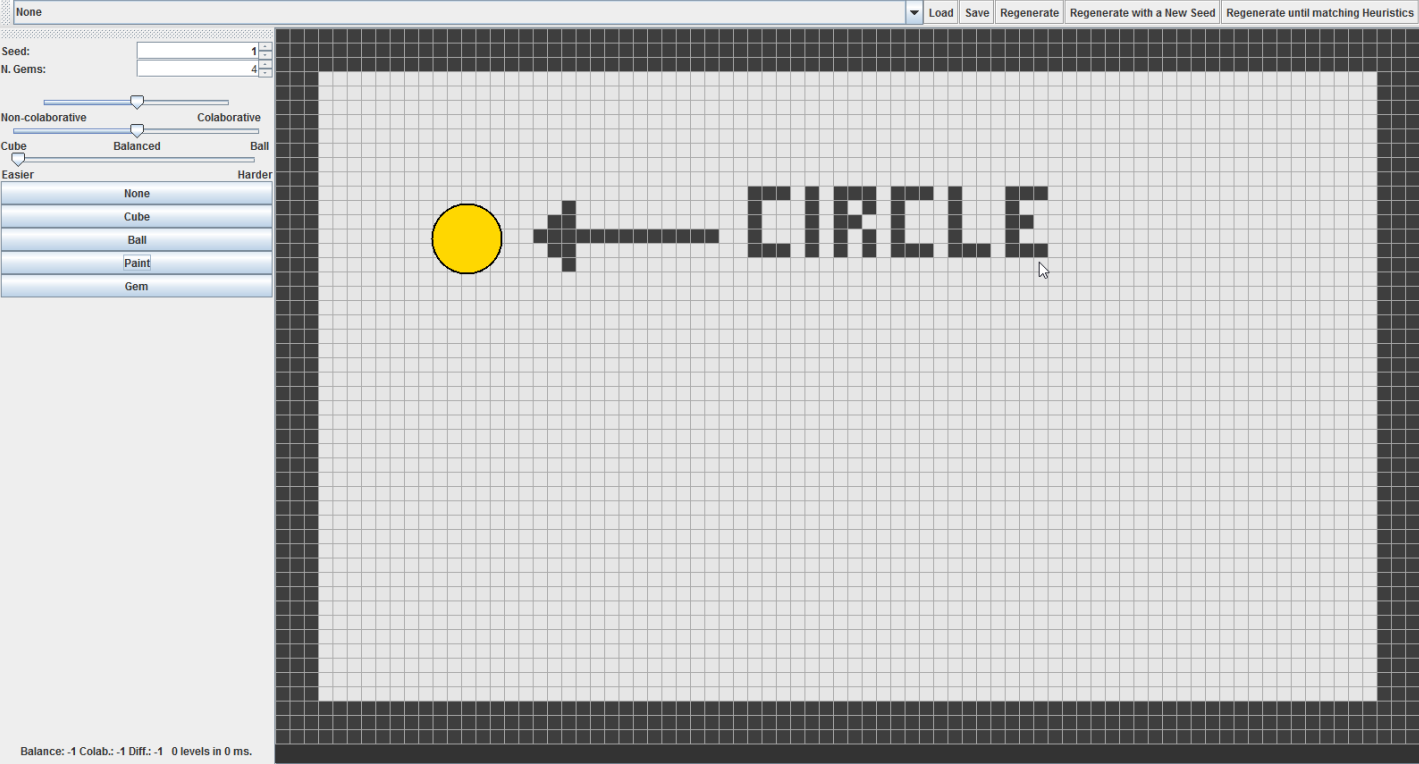
\includegraphics[scale=0.30]{images/rafaeleditor.png}
    \caption{The editor that Rafael created}
    \label{fig:rafaeleditor}
\end{figure}

These heuristic acted more as a threshold and less as a sum of different features, becuase to decide where it would place the collectibles it would take the desired values from the heuristic, and a seeded pseudo random number generator, it would generate a random value and compare it to the collaboration value, if the random value was lower it would place a collectible in the cooperative exclusive zone. If it was greater it would place one in either the circle or the rectangle exclusive zones, the zone where it would generate one would be based on another generated value that would then be compared to the balance heuristic, if it was greater then it would place it on a rectangle exclusive zone. This process would be repeated until there were no more collectibles to place. 
 
These heuristics have a value defined by the designer so they are not directly calculated but we can look at the collaboration heuristic as:
\begin{equation}
hc = \frac{coop - cc - cr}{ C} 
\end{equation}
where \textit{C} is the total number of collectibles, \textit{coop} is the number of collectibles in the cooperative exclusive zone, \textit{cc} is the number of collectibles in the circle exclusive zone and \textit{cr} is the number of collectibles in the rectangle exclusive zone. This heuristic varies between -1 and 1 where -1 does not require any cooperation and 1 means every collectible requires cooperation to be caught. 

And we can look at the balance heuristic as:
\begin{equation}
hb = \frac{cc - cr}{ C} 
\end{equation}
This heuristic varies between -1 and 1 where -1 does means every non cooperative collectible is in the rectangle exclusive zone and 1 is when those collectibles are all in the circle exclusive zone.

Pedro~\cite{ref_thesispedro} attempted to generate levels by using Monte Carlo Tree Search (MCTS). He used it to create an agent whose objective was to create a level in geometry friends using the platforms that where given to it. The MCTS algorithm requires 4 things, the actions the player can do, a deterministic world, the game over condition, and the winning condition. For the actions he defined them as "placing a platform in the X and Y coordinates" each action would have a varying X and Y. While MCTS works better with a deterministic world there are methods to counteract non-determinism in a world, normally through repeating a part of the process. Still in this case the world can be represented in a deterministic way, and so he defined it as a grid. The end condition was determined to be when there were no more platforms to place in the level. The success condition was defined using a score, so that there could be better or worse levels. Pedro based his evaluation on the heuristics from Rafael~\cite{ref_thesisrafael}, using the base structure and implementation of his work, but changing the balance, considering that a level is balanced only if there is at least one collectible in each exclusive area. This was to guarantee a need for cooperation while having an equilibrium between both players. The score could then be 0 if the level is not playable, 1 is playable but does not cooperation to be completed, 2 is when the level required cooperation to be beaten, but might not be balanced, 3 is when a level has cooperation, and is balanced, therefore the best possible score.

The final generator had a level editor that would allow the designer to add platforms by drawing their shape, alternatively it allowed for completely random platforms to be generated. Finally the designer could press a button to generate the level and it would appear in the editor.

\section{Proposed Solution}
In this section we will describe how we plan on creating a procedural cooperative level generator for the game Geometry Friends.

The generator we want to create is focused on mixed authorship, much like the previous attempts there where level editors, however these had the user create the platforms, or they would simply place the collectibles. What we want is to give the designer the ability to give a different type of information, such as an overview of a possible solution of the level.

Our approach is to create an algorithm that uses information about the solution provided by the designer. One type of input would be a step by step solution of how to complete the level, they would indicate where each character starts and then define a sequence of actions that each would do, describing how they would move, where they would use an ability, where they would interact with objects in the map, and where and when they would interact with each other. We want to attempt this solution to help guaranty reliability, because there would always be at least one solution.

Another type of input would have the designer providing an overview of the solution, they would indicate where each character starts, which objectives in the map have to be completed using cooperation and which can or have to be individual, they could even select areas of the level where they would want a cooperative action to take place, or, for example, an area where only the rectangle could go.

When looking at the properties defined previously we can see that for our approach, the levels will be generated before hand so Speed is not as important, it has to be possible to complete a level so we need it to be highly reliable. Seeing as we want the Designer to be able to control the output and input we need a high degree of controllability, hence the editor. As for expressivity and diversity there needs to be variation between the different levels, for example, if we give the same input we might want to be capable of generating different levels.

To develop our solution we will follow a sequence of objectives. First we have to define a language to represent the input that specifies a solution, then we create the algorithm that using that language generates the levels, next we have to develop a tool to allow the editor to use that language, then we would expand the original language to include more abstract representations of the solution.

For our initial language when describing the solution a move action could be a colored, green for rectangle and yellow for circle, arrow to right or left, indicating they have to move to that position. Then a jump action would need to have a direction as well, for this we can use a curve that shows the trajectory the jump would need to take, since the jump from a circle always reaches its highest point, the curve would only differentiate in openness. As for the rectangle its extend action, that allows it to extend vertically or horizontally, to indicate it we can use a line that would represent the height it needs to have in that certain part of the level where the line was placed. All these actions could have numbers attached to them, indicating when they would need to be done.

After having the input solution we can create different sets of steps, then we would place a collectible at the last step of each set and we then consider each set as a level. Next using a shape grammar we place platforms in such a way that the collectible is accessible, this way we can generate simpler levels, that contain only a part of the desired solution, on which we can explore variations using genetic algorithms. We can then create different offspring by crossing the platforms and collectibles, this way we are over time combining all steps given in the input. The fitness function will prefer the levels that have only reachable collectibles and that promote cooperation while having a balanced distribution of actions between the players, for this we will use the definition of balance Pedro used, of having a collectible in each exclusive zone. To test whether a level is possible to complete we will use the approach Rafael developed to determine the exclusivity zones and check if the collectibles are inside those zones, if they are not then it means they are unreachable. We combine levels until the new offspring does not differ much from the previous.

To expand our language we would need more tools to describe the solution, these tools would be much like platforms, but they would represent areas, such as the previously defined, circle only area, rectangle only area, cooperative area and common area. If some areas of the level are left undefined then we could either consider them as common areas or unreachable areas where no character is meant to reach. We can also look at overlapping of areas and in that case we consider them as a hierarchy where the cooperative area is the most important and the common area the least, alternatively an overlap of the circle only and rectangle only can be seen as a cooperative area, or a common area. We would also add a way to specify cooperative actions, such as the circle goes on top of the rectangle and then the rectangle has to expand so the circle can reach higher, or the circle goes on top of the rectangle and the rectangle moves sides ways through platforms on which the circle can not stand such as the yellow platforms.

In another more simpler look at representing a level, we could use colored collectibles, purple diamonds would be collectibles any character could reach, yellow diamonds could only by acquired by the circle, green by the rectangle, and blue would require cooperation between both players.

\section{How to evaluate it}
We plan on testing this approach by allowing users to try the new editor, to see if using a mixed authorship approach is intuitive, and through feedback see if this could be an approach for other games. The next step is to evaluate the levels themselves, so we will start by having the players play an introductory level, and then we will choose among the many already created levels, and add them to a pool with levels generated by our approach. We will then ask if they could tell which where created by our generator. We will also have them classify each on how they felt the levels where in terms of cooperation and individual actions.

We will evaluate our generator based on reliability, i.e. if all levels created can be beaten, on expressivity and diversity, i.e. if the levels are varied and different, quality of levels, and resource consumption, i.e. how much computer memory it requires, how long it takes to generate a level and how much it requires from the cpu.

\section{Work Schedule}

\begin{figure}
    \centering
    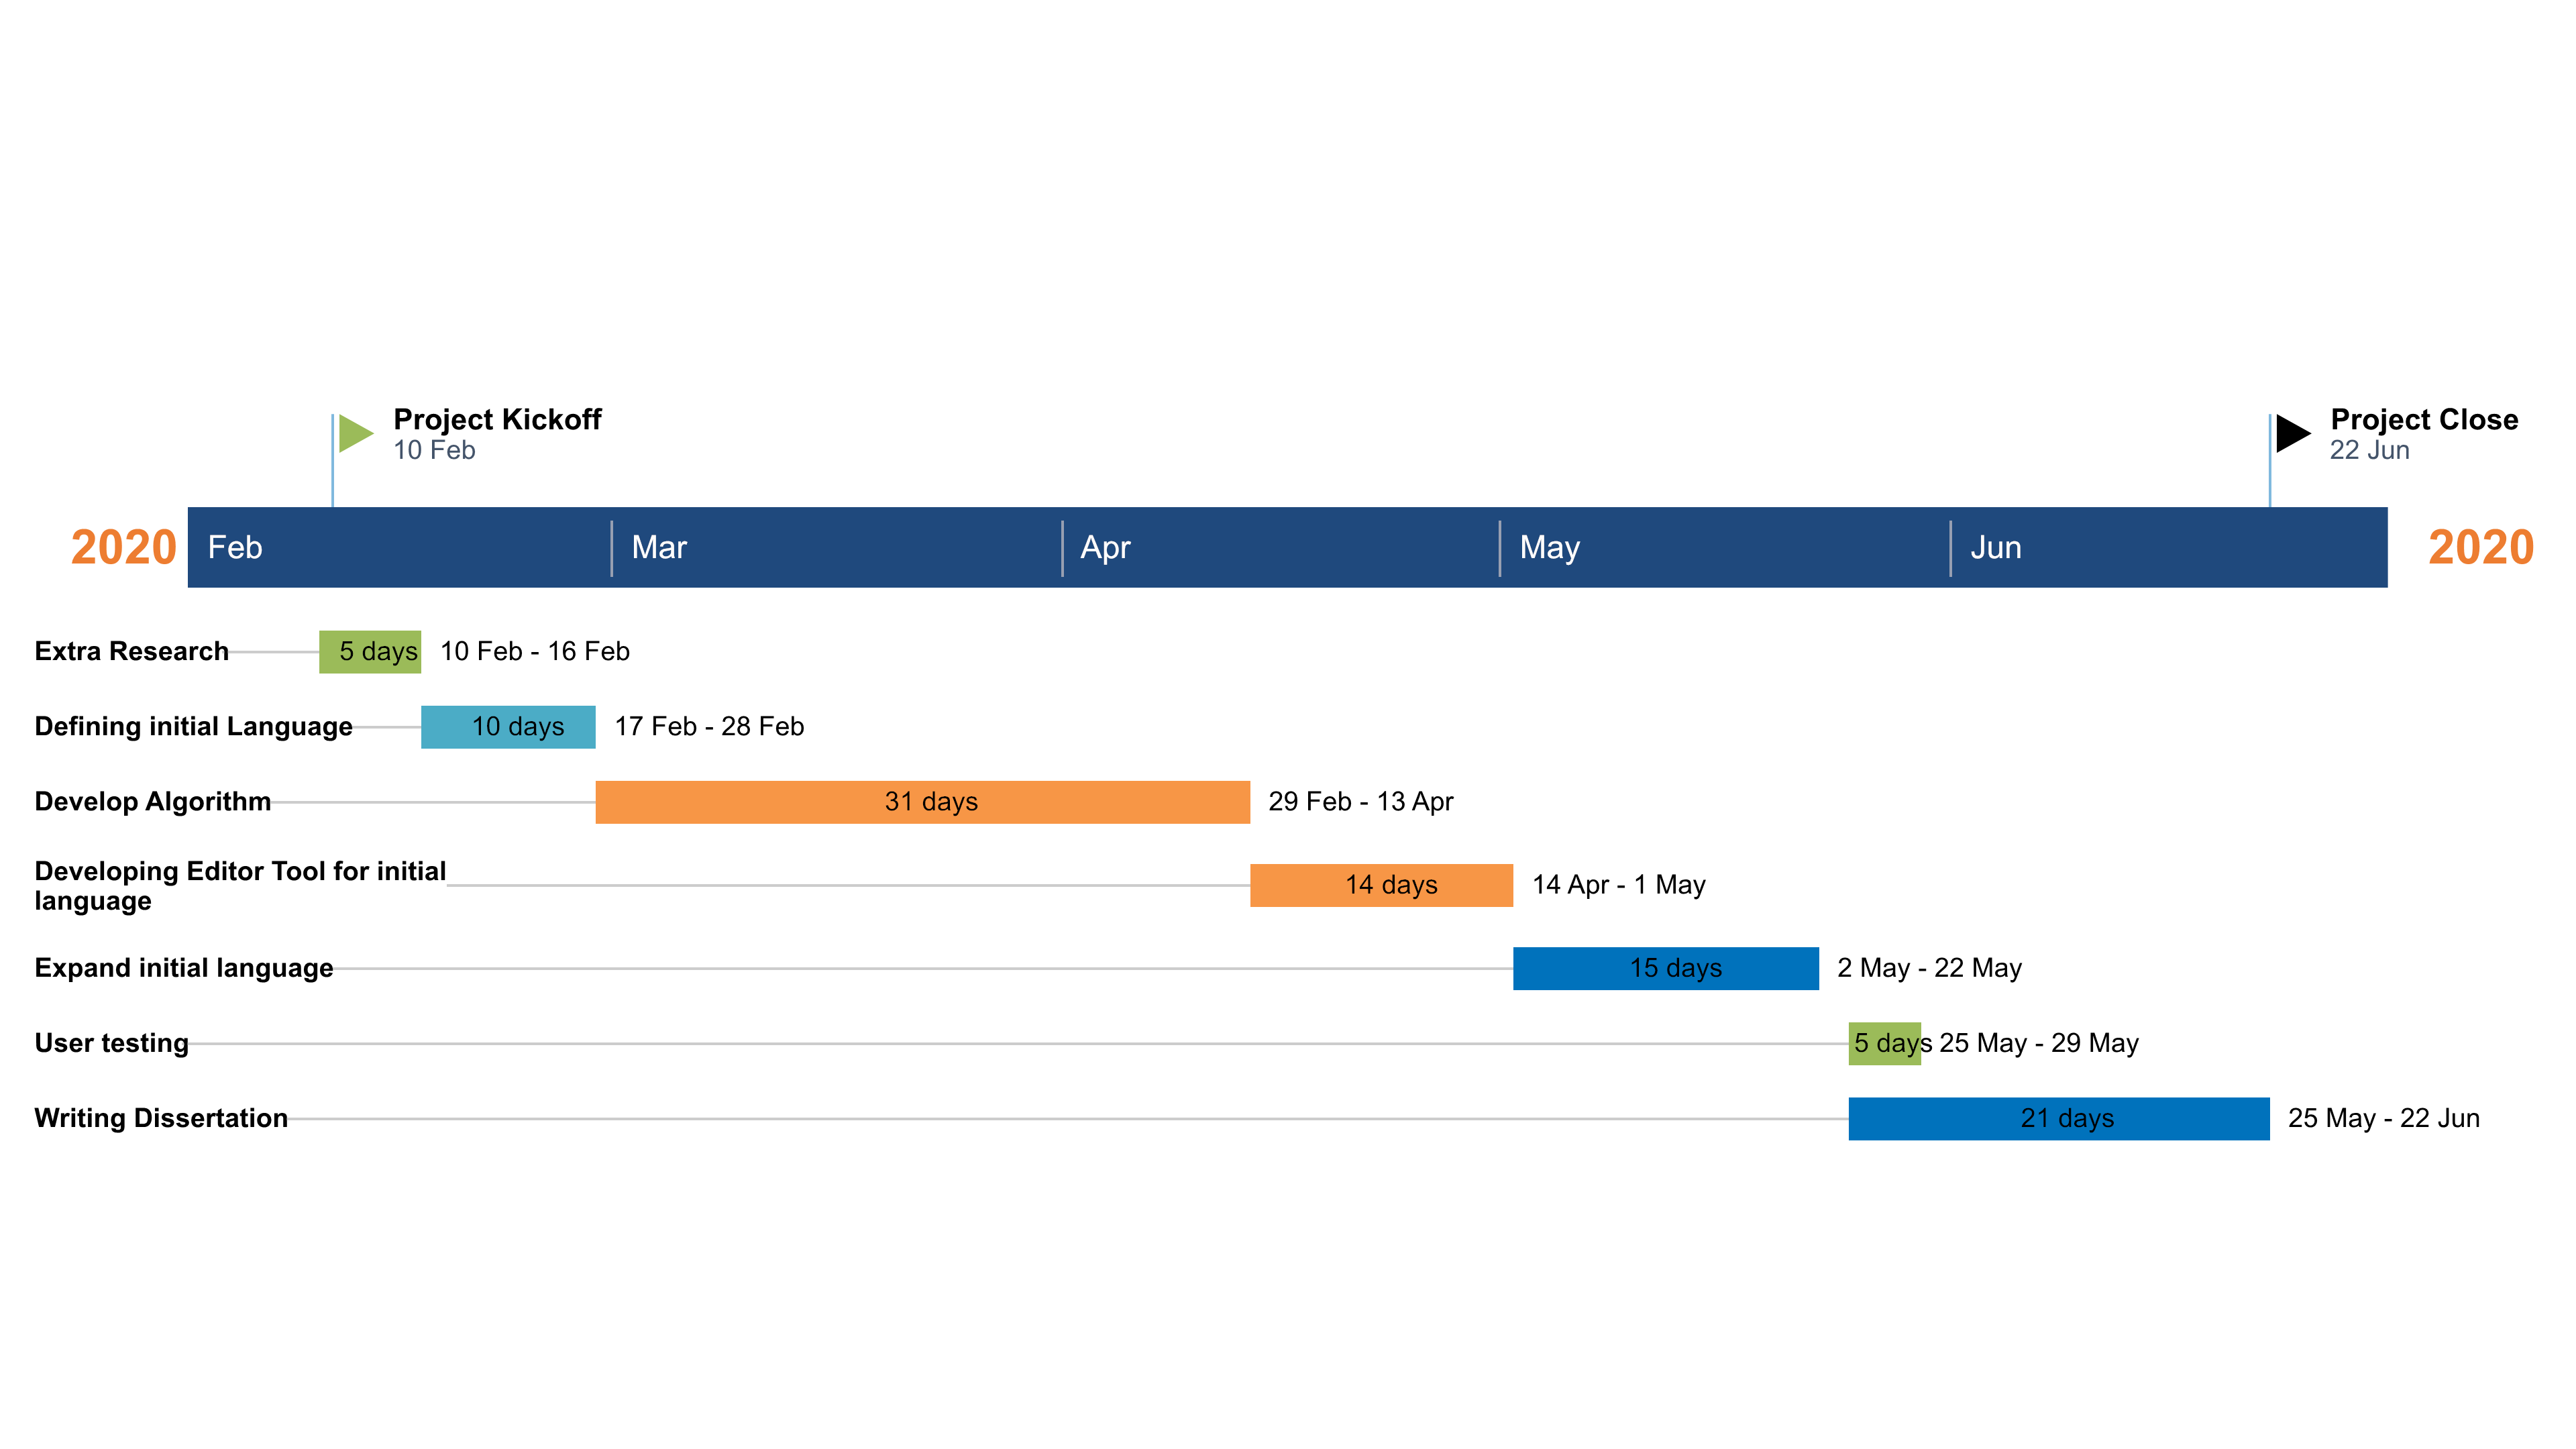
\includegraphics[scale=0.109]{images/gantt.png}
    \caption{Work Schedule}
    \label{fig:gantt}
\end{figure}

\section{Conclusion}

We explored the state of the art in procedural content generation and cooperative game design, we found that very little research has gone into procedural content generators that promote cooperation in games. We show Geometry Friends as a good test bed for Procedural Cooperative Content Generators, having had two previous generators created. We propose a new solution for this problem that aims at generating a level based on a solution for said level.

\begin{thebibliography}{40}

\bibitem{ref_togelius}
Noor Shaker, Julian Togelius, and Mark J. Nelson. 2016. Procedural Content Generation in Games (1st ed.). Springer Publishing Company, Incorporated.

\bibitem{ref_hendrikx}
Hendrikx, M., Meijer, S., van der Velden, J., and Iosup, A. 2011. Procedural Game Content Generation: A Survey. ACM Trans. Multimedia Comput. Commun. Appl. -, -, Article 1 (February 2011), 24 pages. DOI = 10.1145/0000000.0000000 http://doi.acm.org/10.1145/0000000.0000000

\bibitem{ref_rocha}
Rocha, J.B., Mascarenhas, S., Prada, R.: Game mechanics for cooperative games. 

\bibitem{ref_magy}
Magy Seif El-Nasr, Bardia Aghabeigi, David Milam, Mona Erfani, Beth Lameman, Hamid Maygoli, and Sang Mah. 2010. Understanding and evaluating cooperative games. In Proceedings of the SIGCHI Conference on Human Factors in Computing Systems (CHI '10). ACM, New York, NY, USA, 253-262. DOI: https://doi.org/10.1145/1753326.1753363

\bibitem{ref_smith}
Smith, G. (2015). An Analog History of Procedural Content Generation. FDG.

\bibitem{ref_arkel}
van Arkel, B., Karavolos, D., and Bouwer, A. (2015). Procedural generation of collaborative puzzle-platform game levels. In S. Bakkes, and F. Nack (Eds.), GAME-ON' 2015: 16th International Conference on Intelligent Games and Simulation (pp. 87-93). Amsterdam: Eurosis.

\bibitem{ref_zagal}
Zagal, Jose and Rick, Jochen. (2006). Collaborative games: Lessons learned from board games. Simulation and Gaming - Simulat Gaming. 37. 24-40. 10.1177/1046878105282279. 

\bibitem{ref_dormans}
Dormans J., 2012. Engineering emergence: Applied theory for game design. Ph.D. thesis, University of Amsterdam.

\bibitem{ref_thesisrafael}
Rafael Vilela Pinheiro de Passos Ramos, November 2015, Procedural Content Generation for Cooperative Games, MSc in Information Systems and Computer Engineering, Instituto Superior Técnico

\bibitem{ref_thesispedro}
Pedro Costa Borges, May 2018, Procedural Content generation for Cooperative Games, MSc in Information Systems and Computer Engineering, Instituto Superior Técnico


%%% Have not read, but were referenced by other papers in that specific context

\bibitem{ref_reuter}
Reuter C.; Wendel V.; Göbel S.; and Steinmetz R., 2014.Game Design Patterns for Collaborative Player Interactions. DiGRA 2014 (accepted for publication)

\bibitem{ref_whitehead}
Hullett K. and Whitehead J., 2010. Design patterns in FPS levels. In proceedings of the Fifth International Conference on the Foundations of Digital
Games. ACM, 78–85.

\bibitem{ref_patel}
Patel, A. 2010. Polygonal map generation. Blog www-cs-students.stanford.edu/\texttildelow amitp/game-programming/polygon-map-generation/.

\bibitem{ref_pell}
Pell, B. 1993. METAGAME in symmetric chess-like games. Tech. Rep. UCAM-CL-TR-277, University of Cambridge, Computer Laboratory

\bibitem{ref_schmidhuber}
Togelius, J. and Schmidhuber, J. 2008. An experiment in automatic game design. In IEEE Symposium on Computational Intelligence and Games, 2008. CIG’08. IEEE, 111–118.

\bibitem{ref_hom}
Hom, V. and Marks, J. 2007. Automatic design of balanced board games. In Proc. 3rd Artificial Intelligence and Interactive Digital Entertainment Conference. 25–30.

\bibitem{ref_brathwaite}
Brenda Brathwaite and Ian Schreiber. 2008. Challenges for Game Designers (1 ed.). Charles River Media, Inc., Rockland, MA, USA.

\bibitem{ref_mateas}
Smith, A. M. and Mateas, M. 2010. Variations Forever: Flexibly generating rulesets from a sculptable design space of minigames. In IEEE Symposium on Computational Intelligence and Games (CIG). IEEE, 111–118.

\bibitem{ref_hartsook}
Hartsook, K., Zook, A., Das, S., AND Riedl, M. Toward supporting stories with procedurally generated game worlds.

\bibitem{ref_chan}
Chan, C., Thawonmas, R., and Chen, K. 2009. Automatic storytelling in comics: a case study on World of Warcraft. In International Conference on Human factors in computing systems. ACM, 3589–3594.

\bibitem{ref_perlin}
Perlin, K. 1985. An image synthesizer. SIGGRAPH Comput. Graph. 19, 287–296.

\bibitem{ref_verth}
James M. Van Verth and Lars M. Bishop. 2008. Essential Mathematics for Games and Interactive Applications, Second Edition: A Programmer's Guide (2 ed.). Morgan Kaufmann Publishers Inc., San Francisco, CA, USA.

\bibitem{ref_stiny}
Stiny, G. 1975. Pictorial and Formal Aspects of Shape and Shape Grammars. Birkhauser Verlag, Basel.

\bibitem{ref_wonka}
Peter Wonka, Michael Wimmer, François Sillion, and William Ribarsky. 2003. Instant architecture. ACM Trans. Graph. 22, 3 (July 2003), 669-677. DOI: https://doi.org/10.1145/882262.882324

\bibitem{ref_larive}
Mathieu Larive and Veronique Gaildrat. 2006. Wall grammar for building generation. In Proceedings of the 4th international conference on Computer graphics and interactive techniques in Australasia and Southeast Asia (GRAPHITE '06). ACM, New York, NY, USA, 429-437. DOI=http://dx.doi.org/10.1145/1174429.1174501

\bibitem{ref_franz}
Franz Aurenhammer. 1991. Voronoi diagrams—a survey of a fundamental geometric data structure. ACM Comput. Surv. 23, 3 (September 1991), 345-405. DOI=http://dx.doi.org/10.1145/116873.116880

\bibitem{ref_pi}
Pi, Xuexian and Song, Junqiang and Zeng, Liang and Li, Sikun. (2006). Procedural Terrain Detail Based on Patch-LOD Algorithm. 3942. 913-920. 10.1007/11736639\_111. 

\bibitem{ref_chopard}
Chopard, B. and Droz, M. 1998. Cellular Automata Modeling of Physical Systems. Cambridge University Press.

\bibitem{ref_chentensor}
Chen, G., Esch, G., Wonka, P., Muller , P., and Zhang, E. 2008. Interactive procedural street modeling. In ACM SIGGRAPH 2008 Papers. ACM, 103.

\bibitem{ref_davidsson}
Davidsson, P. 2001. Multi agent based simulation: Beyond social simulation. In Multi-Agent-Based Simulation, S. Moss and P. Davidsson, Eds. Lecture Notes in Computer Science Series, vol. 1979. Springer Berlin / Heidelberg, 141–155. 

\bibitem{ref_goldberg}
David E. Goldberg. 1989. Genetic Algorithms in Search, Optimization and Machine Learning (1st ed.). Addison-Wesley Longman Publishing Co., Inc., Boston, MA, USA.

\bibitem{ref_haykin}
Simon Haykin. 1994. Neural Networks: A Comprehensive Foundation (1st ed.). Prentice Hall PTR, Upper Saddle River, NJ, USA.

\bibitem{ref_russel}
Russel, S., Norvig, P., Canny, J., Malik, J., and Edwards, D. 1995. Artificial intelligence: a modern approach. Vol. 74. Prentice hall Englewood Cliffs, NJ.

\end{thebibliography}
%
%\begin{gamereferences}{30}
%Games all in the end
%\bibitem{ref_civilization}
%Firaxis, 2K Games 2011, Civilization VI, video game, Microsoft Windows, United %States.
%
%\bibitem{ref_nomanssky}
%Hello Games 2016, No Man's Sky, video game, Microsoft Windows, United Kingdom.
%
%\bibitem{ref_minecraft}
%Mojang 2009, Minecraft, video game, Microsoft Windows, Mojang, Sweden. 
%
%
%\bibitem{ref_terraria}
%Re-Logic 2011, Terraria, video game, Microsoft Windows, Re-Logic, Indiana, %United States.
%
%\bibitem{ref_spelunky}
%Derek Yu 2008, Spelunky, video game, Microsoft Windos, Derek Yu.
%
%\bibitem{ref_left4dead}
%Turtle Rock Studios 2008, Left 4 Dead, video game, Microsoft Windows, Valve, %United States.
%
%\bibitem{ref_thebindingofisaac}
%Edmund McMillen 2011, The Binding of Isaac, video game, Microsoft Windows, %Edmumd McMillen.
%\end{gamereferences}
%


\end{document}
